\chapter{Asking Billionaires How They Got RICH! (Boston)}

These notes follow the progression of a School of Hard Knocks interview in Boston and are prepared for this book project under the curation of LazyingArt LLC. The lecture itself contains no blackboard mathematics, but it does contain a great deal of quantitative language, and that language can easily be misread if we do not separate its objects. The opening montage alone throws annual salary, company valuation, and founder-scale wealth into one visual field. Our task is therefore not to force a textbook onto the interview, but to keep its categories straight while preserving the order in which the speaker uncovers them.

\section{Boston as a Wealth Field}

The lecture begins in compressed form. We are shown three ways of becoming rich: athlete wealth, inventor wealth, and product-company wealth. Then, before any system is extracted from the examples, the montage closes with a warning: if the ambition is simply to become a billionaire, good luck. That warning is not a flourish. It is the lecture's first filtering principle. The city will supply examples of wealth, but the chapter will repeatedly insist that wealth itself is not yet an adequate aim.

Only after this teaser does the lecture settle into its true first move. Boston is presented as a comparative money field, a city dense enough in capital and institutions that several wealth mechanisms can be sampled in a single outing. The demographic anchor is modest but useful:
\begin{equation}
N_{\text{millionaires,Boston}} > 40{,}000,
\qquad
N_{\text{billionaires,Boston}} > 10.
\end{equation}

Now the bookkeeping must begin. The interview speaks loosely of ``money,'' but the cases that follow involve distinct quantities:
\begin{align}
Y &:= \text{annual personal earnings},\\
V &:= \text{company valuation},\\
A &:= \text{assets under management},\\
W_t &:= \text{investable wealth at time } t.
\end{align}
One of the chapter's quiet obligations is to keep these from collapsing into one another. A salary is not a valuation. A valuation is not liquid personal wealth. Assets under management are not the same thing as ownership. The lecture gains clarity once this is admitted.

\begin{remark}
Because the interview offers no visible board mathematics, every formula in this chapter is a disciplined reconstruction. We use notation only where it clarifies the underlying mechanism rather than replacing it.
\end{remark}

\section{Whoop: Problem First, Company Second}

The first sustained case is the founder of Whoop. The host begins in the standard register of the series by asking when he became a millionaire, but the answer quickly diverts us toward a more instructive question: what was he trying to do before he was trying to become wealthy? The founder's answer is decisive. He did not begin with the abstract ambition ``I want to start a company.'' He began with a concrete ambition: to understand health, to build wearables, and to create devices that millions of people could use to improve their health. The problem precedes the company.

The quantitative markers are straightforward:
\begin{equation}
t_0 = 2012,
\qquad
T_{\text{build}} \approx 12\ \text{years},
\qquad
V_{\text{Whoop}} \approx \$3.6 \times 10^9.
\end{equation}
The point, however, is not the size of \(V_{\text{Whoop}}\). The point is the order of construction. First the problem; then the long build; only much later the valuation language that outsiders prefer.

This matters because the lecture briefly tempts us to read entrepreneurship as temperament. Did he always know he would work for himself? Was entrepreneurship innate? The answer, as the notes should preserve, is subtler. He may have known he did not wish to work for others, but the stronger claim is that the problem did the real organizing work. That is the narrative lever by which the lecture moves from biography into method.

\begin{definition}
A signal event is a publicly visible fact that is small in immediate cash consequence but large in informational consequence. It changes the founder's estimate that the business may in fact be real and survivable.
\end{definition}

The Whoop story gives us such an event. By 2015 the company is still struggling, yet LeBron James appears in a Kia commercial wearing a Whoop. At that moment the installed base is extremely small:
\begin{equation}
N_{\text{Whoop straps at the LeBron moment}} \approx 100.
\end{equation}
That number is what makes the event mathematically interesting. One does not merely observe celebrity usage. One observes celebrity usage against a background of near nonexistence. A single device among roughly one hundred has reached the most visible athletic tier in the world. The lecture treats this not as revenue, but as proof that the firm has touched reality.

\begin{figure}
\centering
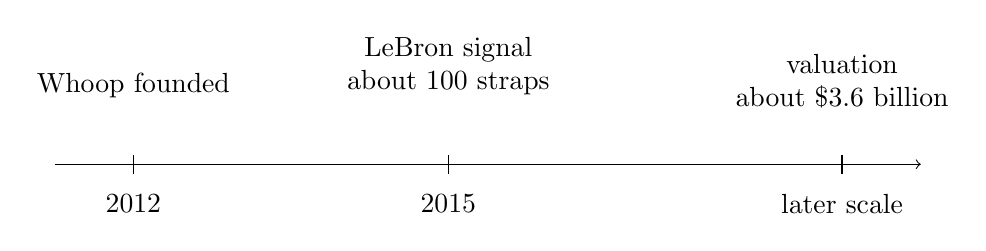
\begin{tikzpicture}[x=1cm,y=1cm]
\draw[->] (0,0) -- (11,0);
\draw (1,0.12) -- (1,-0.12);
\draw (5,0.12) -- (5,-0.12);
\draw (10,0.12) -- (10,-0.12);
\node at (1,-0.5) {2012};
\node at (5,-0.5) {2015};
\node at (10,-0.5) {later scale};
\node[align=center] at (1,1.0) {Whoop founded};
\node[align=center] at (5,1.25) {LeBron signal\\about \(100\) straps};
\node[align=center] at (10,1.05) {valuation\\about \(\$3.6\) billion};
\end{tikzpicture}
\end{figure}

The timeline reminds us that the lecture resists the clean founder myth. Between \(t_0\) and the later valuation there is a middle region in which the company is neither obviously dead nor obviously secure. That middle region is where the next section lives.

\section{Courage Under Liquidity Stress}

The lecture now tightens the screw. The host asks for a lesson not taught at Harvard Business School. The answer is striking because it bypasses the usual founder vocabulary. Not vision, not strategy, not empathy, not business acumen, but courage. This is the point at which the interview stops sounding like a success story and starts sounding like a study of binding constraints.

We can encode the founder's own description of the strain in a minimal schematic:
\begin{equation}
K_t \downarrow,
\qquad
P_t\ \text{due},
\qquad
q_t\ \text{uncertain}.
\end{equation}
Here \(K_t\) denotes cash or runway, \(P_t\) denotes payroll and other immediate obligations, and \(q_t\) denotes the state of the product. The transcript gives us all three pieces in ordinary language: the company almost ran out of money, almost missed payroll, and had moments in which the product was failing. Six or seven years into the build, the founder still describes himself as broke.

\subsection{Question \& Answer}

\paragraph{Question.} What is the hardest trait in building a company when things are actually going wrong?

\paragraph{Answer.} The lecture's answer is courage. Not theatrical courage, but managerial courage: the willingness to say the hard thing, do the hard thing, and step into the problem instead of standing outside it. Strategy still matters, of course. But strategy without the willingness to own the crisis remains inert.

The order is crucial. The lecture first states the claim about courage and only then supplies the evidence: near failure, binding payroll, product weakness, and the temptation to quit. In this sense the answer is not a slogan attached to success after the fact. It is the proposed explanation for why the firm was not abandoned while it was still weak.

The LeBron event re-enters here as morale rather than money. It does not erase the system
\[
K_t \downarrow,\qquad P_t\ \text{due},\qquad q_t\ \text{uncertain},
\]
but it alters the founder's belief that persevering may still be rational. One can say it this way: the signal event does not solve the company, but it changes the founder's posterior estimate that the company deserves another round of effort.

The lecture immediately adds one more beat. Entrepreneurship is not for everyone. It is, in the founder's language, a lesson in pain and suffering for a greater cause. That line belongs here because it is the natural consequence of the previous equation. If the central region of the enterprise is exactly the region in which cash is thin, payroll is binding, and the product is not yet fully proven, then one should not romanticize entry into that region.

\section{Product, Competition, and the Distribution Illusion}

Having shown us that the business can be attacked from within, the lecture now turns to the external threat: competition. The question is direct. What happens when a much larger company enters the field? Here again the lecture refuses a simple slogan. The founder does not say that competition is imaginary, nor does he say that sheer size guarantees victory. Instead he states a more discriminating claim: large distribution is not the same thing as durable adoption.

The reconstructed causal contrast is therefore modest:
\begin{align}
\text{distribution alone} &\not\Rightarrow \text{durable success},\\
\text{distribution} + \text{product quality} &\Rightarrow \text{repeat use and loyalty}.
\end{align}

The Whoop founder describes the product as integrated, data-rich, and associated with a distinct brand. The Amazon episode, though slightly rough in transcription, has a clear structure. A copycat product appears. It has access to large distribution. Yet it fails because it lacks the specific quality that makes people want to wear it. The lecture calls this the missing ``magic.'' We should not overformalize that term; still, it names a real point. A copied shell is not the same as a loved object.

\subsection{Question \& Answer}

\paragraph{Question.} What beats large distribution: scale or a product that people actually love?

\paragraph{Answer.} The answer is neither sentimental nor naive. Scale matters, and the founder explicitly says it was taken seriously. But scale by itself is not the decisive variable. The decisive variable is whether the product has enough internal quality that people continue to use it. In the lecture's rhetoric, the larger firm can copy the exterior and still miss the reason the original worked.

The section closes with the founder's compressed blueprint: find something you love, become obsessed with it, drop entitlement, do hard work that others are unwilling to do, persist, build a great team, raise capital, and keep going. The notes should preserve the sequence here. The blueprint is given only after the lecture has exposed the costs of following it.

\section{Jalen Brown: Adversity, Money, and the Interior Game}

The next segment changes the grammar of wealth without leaving the subject of wealth. The host meets Jalen Brown at MIT and first asks not about money, but about the factor behind his success as an athlete. Brown's answer is adversity and failure. This is an important restoration of order. The lecture does not first ask Brown how much he made and then backfill a philosophy. It first asks what formed him.

Adversity, in Brown's account, is productive. Failure unlocks work ethic, discipline, and creativity. Only after that philosophical claim does the interview turn toward money:
\begin{equation}
Y_{\text{Brown,last year}} \approx \$5.0 \times 10^7.
\end{equation}
Even here, however, the lecture refuses to let \(Y_{\text{Brown}}\) dominate the section. Brown says he does not keep a lot of money in the bank, and adds that rich people often understand that money is just paper. He then introduces another target altogether: social capital.

We should be careful here. Social capital is not formalized in the lecture and should not be forced into a spurious equation. But the logic is clear. A high \(Y\) does not tell us what one values, how one negotiates, or whether one acts from freedom or from desperation. Brown says that he can run away from a deal that does not align with him. Non-desperation, then, becomes a form of wealth that is not reducible to cash balances.

The lecture widens further. Brown speaks about a single-parent household, periods of material shortage, and the ability to provide for family. Then he turns to hatred, imitation, and a line the notes should preserve exactly in spirit: the moon steals light from the sun, but people do not confuse the two. That is the lecture's answer to the problem of imitation. The source remains the source.

From there the interview descends into doubt, anxiety, depression, and dark mental places. This descent is necessary. It keeps the chapter from mistaking public visibility for inner settlement. High income does not remove darkness; at most it changes its surroundings. Brown's final response is neither technical nor financial. It is faith, consistency, and hard work.

\paragraph{A brief interlude on writing.} Before the next interview, the host inserts a short aside on business writing. Opportunity often begins with an email; writing is how one pitches, leads, hires, and connects. This should not dominate the chapter, but it does belong to the lecture's rhythm. After a section on performance and inner life, the talk briefly returns to technique, this time at the level of language.

\section{The Hedge-Fund Operator: Scale, Simplicity, and End Use}

The next interview brings in yet another category:
\begin{equation}
A_{\text{managed}} \approx \$4.0 \times 10^{10}.
\end{equation}
We are now in the world of institutional capital. The speaker reports roughly twenty-one years at a hedge fund, service as a senior partner, and management at the level of about forty billion dollars. But, characteristically, the lecture does not permit this scale to remain abstract. The speaker immediately moves backward into biography: poverty, the projects in Inglewood, a trailer in rural North Carolina, a series of people who invested in him, and a succession of breaks that mattered because he worked hard enough to use them.

Before the investment advice arrives, the lecture inserts one more practical principle. Learn how to dribble with your left. In context, the meaning is plain: do not rely only on what comes naturally. Develop the capacities that are not automatic. This line belongs here because the financial advice that follows is also an argument against vanity. It asks for disciplined simplicity rather than ego-driven cleverness.

\subsection{Question \& Answer}

\paragraph{Question.} Where should most people put their money if they know less than they think they know?

\paragraph{Answer.} The answer is intentionally ordinary: a low-cost index fund, and specifically the S\&P 500 through a provider such as Vanguard. The underlying principle is epistemic modesty. Intelligent people know what they know and what they do not know. For most households, broad exposure and patience are better than improvised brilliance.

To write this cleanly, we use the standard compounding recurrence
\begin{align}
W_{t+1} &= (1+r)W_t + s_t,\\
W_0 &= 0,
\end{align}
where \(W_t\) is investable wealth at time \(t\), \(r\) is the period return of the broad index vehicle, and \(s_t\) is the net contribution during the period. This is not a quoted lecture formula. It is the minimal mathematical structure required to express the compounding logic the speaker is invoking.

\paragraph{Worked example.} Suppose \(s_t=s\) is constant. Then
\begin{align}
W_1 &= s,\\
W_2 &= (1+r)s + s,\\
W_3 &= (1+r)^2s + (1+r)s + s.
\end{align}
Hence
\begin{equation}
W_n = s\sum_{k=0}^{n-1}(1+r)^k
    = s\,\frac{(1+r)^n-1}{r}.
\end{equation}
This is the clean mathematical version of the lecture's anti-complication advice. One does not need secret brilliance to begin compounding. One needs a simple vehicle, repeated contributions, and time.

But once again the lecture refuses to stop at the formula. When the host asks about the most money made in a year, the speaker redirects the measure toward giving. When asked whether money buys happiness, the answer is no: money makes one more of what one already is. Then come faith, mortality, and marriage. The best financial decision, in this section, is not a market trade at all, but the choice of an extraordinary partner whose character supports a life of shared growth.

The section's final aphorism should remain verbal rather than algebraic: self-interest is essential, selfishness is not. The lecture wants practical finance and moral orientation to occupy the same page.

\section{Jim Cook: Selling, Scarcity, and Control}

The Samuel Adams interview is the lecture's fullest founder case after Whoop, and it ends up restating the chapter's entire thesis from another angle. The host first asks how Jim Cook got rich and is told, with deliberate plainness, that he created the listener's favorite beer. The scale line that follows --- ``like \$2$ billion'' in a single year --- should be handled cautiously as a scale signal rather than a clean income measure. The lecture itself quickly moves on to the more interesting question: what really built the company?

\subsection{Question \& Answer}

\paragraph{Question.} What matters more in a company's rise: branding, selling, or product quality?

\paragraph{Answer.} Jim Cook's answer is sharp. Branding, he says, is not that important; marketing is overrated; what really works is a better product and the hard work of selling it. The notes should keep the force of that claim without inflating it into a universal theorem. It is the doctrine of this founder case, not a law of nature.

The transcript gives us a few numbers that make the argument concrete:
\begin{equation}
\Delta t_{\text{launch}\to\text{best beer}} \approx 6\ \text{weeks},
\qquad
T_{\text{first marketing hire}} \approx 10\ \text{years},
\qquad
N_{\text{salespeople at that point}} = 80.
\end{equation}
These markers are important precisely because they replace slogan with allocation. If the first marketing hire comes only after roughly a decade, while eighty salespeople already exist, then the distinction between marketing and selling is not a retrospective pose. It is part of the operating design.

The naming story reinforces the same lesson. Two names test about equally well. He chooses Samuel Adams, but says the company would likely have done just as well under another name, because the decisive variable was not the label but the beer itself. The company had a better glass of beer.

The lecture then turns to the most life-changing conversation of the section. Jim spends a day worrying about computers and tax savings, and his uncle cuts through the confusion. Many companies have gone broke with computers; they went broke because they had no sales. That is the right moment to introduce the lecture's simplest update rule:
\begin{equation}
N_{t+1}=N_t+1.
\end{equation}
The rule represents the uncle's instruction: get one customer every day and do not come home without one. It is deliberately primitive. It is not a forecast model for a mature firm. It is a discipline rule for an early founder.

If \(N_0=0\), then after thirty days one has
\begin{equation}
N_{30}=30.
\end{equation}
The point is not the number \(30\) in itself. The point is that business movement is being generated by customer contact rather than by endless preparation.

\begin{figure}
\centering
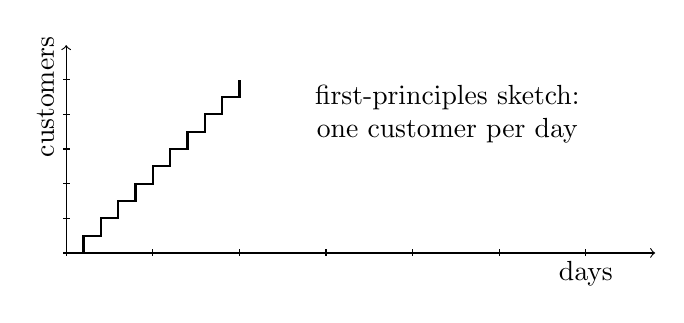
\begin{tikzpicture}[x=0.22cm,y=0.22cm]
\draw[->] (0,0) -- (34,0);
\draw[->] (0,0) -- (0,12);
\foreach \x in {0,5,10,15,20,25,30}
  \draw (\x,0.2) -- (\x,-0.2);
\foreach \y in {0,2,4,6,8,10}
  \draw (0.2,\y) -- (-0.2,\y);
\node at (30,-1.2) {days};
\node[rotate=90] at (-1.2,9) {customers};
\draw[thick] (0,0)
-- (1,0) -- (1,1)
-- (2,1) -- (2,2)
-- (3,2) -- (3,3)
-- (4,3) -- (4,4)
-- (5,4) -- (5,5)
-- (6,5) -- (6,6)
-- (7,6) -- (7,7)
-- (8,7) -- (8,8)
-- (9,8) -- (9,9)
-- (10,9) -- (10,10);
\node[align=center] at (22,8) {first-principles sketch:\\one customer per day};
\end{tikzpicture}
\end{figure}

From there the lecture moves into capital discipline. Jim does not build a brewery; he contracts production. He does not rent an office; he uses bars and pay phones. He removes every fixed cost that can be removed and spends only where the company cannot afford to be second-rate. Great ingredients matter. The best brewmaster matters. Production access matters. Cash scarcity therefore produces a second mathematical marker:
\begin{equation}
e_{\text{brewmaster}} = 0.02.
\end{equation}
Two percent of the company is used where cash would have been insufficient. This is the lecture's cleanest example of substituting equity for immediate cash in order to acquire indispensable expertise.

The argument then advances one step further, from startup scarcity to public-market control:
\begin{equation}
t_{\text{public}} = 1995.
\end{equation}
The lecture's claim is that one may go public without surrendering the company outright. Jim Cook says he kept the voting shares and explicitly states that he sacrificed some economics for control. The cleanest shorthand is therefore
\begin{equation}
C \uparrow \quad \Longrightarrow \quad E \downarrow \ \text{may be accepted},
\end{equation}
where \(C\) denotes control rights and \(E\) denotes purely economic share. Again, this is not a theorem from the interview; it is a compact way of preserving the founder's declared tradeoff.

The last movement of the section matters most. The host asks what principle Jim would leave behind. The answer returns us, in mature form, to the cold-open warning. If one's ambition is simply to become a billionaire, then one is aiming at the wrong object. If instead one wants to make great beer and launch a beer revolution, then one may do very well. Wealth, in this account, is almost an accidental by-product. The real organizing variable is meaningful ambition.

\section{Summary}

The lecture begins by compressing several rich outcomes into one montage, but it spends the rest of its time teaching us not to confuse them. Boston becomes useful because it allows athlete income, startup valuation, institutional capital, and founder control to coexist in one field of vision. Once that happens, we can begin to sort them.

The mathematics in this chapter is deliberately light, but it is not ornamental. It performs three pieces of work. First, it separates unlike quantities: \(Y\), \(V\), \(A\), and \(W_t\). Second, it isolates the founder stress region through the schematic
\[
K_t \downarrow,\qquad P_t\ \text{due},\qquad q_t\ \text{uncertain}.
\]
Third, it preserves the lecture's two most practical update rules:
\[
W_{t+1}=(1+r)W_t+s_t,
\qquad
N_{t+1}=N_t+1.
\]
One governs household compounding under simplicity; the other governs early customer acquisition under pressure.

What remains once the bookkeeping is done is a coherent doctrine. Problem-first entrepreneurship matters more than startup vanity. Courage matters when the firm is not yet safe. Distribution without a loved product is unstable. Broad-market compounding is often better than ornamental cleverness. Selling and product quality matter more than branding theater. Control may be worth giving up economics for. And above all, the lecture refuses to let wealth stand alone as the final variable. Meaning, character, faith, and the use to which money is put remain the larger frame in which all the smaller quantities must finally be read.